\documentclass[12pt, a4paper, titlepage]{report}
\usepackage[spanish]{babel}
\usepackage[utf8]{inputenc}
\usepackage[linesnumbered,lined,boxed,commentsnumbered]{algorithm2e}
\usepackage{enumitem,kantlipsum}
\usepackage{float}
\usepackage{subfig}
\usepackage{comment}
\usepackage{booktabs}% http://ctan.org/pkg/booktabs
\newcommand{\tabitem}{~~\llap{\textbullet}~~}
%%Imágenes
\usepackage{graphicx}
%%Colores de texto 
\usepackage{xcolor}
\usepackage{colortbl}
%%Links
\usepackage[hidelinks]{hyperref}
%%Comentarios
\usepackage{verbatim}
%--------------PARA IMÁGENES EN LÍNEA--------------------%

\newcommand*{\img}[1]{%
    \raisebox{-.3\baselineskip}{%
        \includegraphics[
        height=2.5cm,
        width=3cm,
        keepaspectratio,
        ]{#1}%
    }%
}
%--------------FIN DE IMÁGENES EN LÍNEA------------------%

%------------------ESTABLECER COLORES----------------------%
\definecolor{guindapoli}{RGB}{102, 0, 51}
\definecolor{azulescom}{RGB}{0, 0, 102}
\definecolor{azulclaro}{RGB}{222, 232, 255}
\definecolor{azulfuerte}{RGB}{60, 150, 250}
%------------------FIN DE COLORES------------------%

%---------------------------GLOSARIO----------------------------%
\usepackage{glossaries}
% \makeglossaries

% \newglossaryentry{Flash}
% {
%     name=Flash,
%     description={Aplicación informática englobada en la categoría de reproductor multimedia}
% }

%------------------FINAL DE GLOSARIO-----------------------%


\begin{document}
	
	%PARA QUE DETECTE HASTA SUBSUBSECTION
	\setcounter{secnumdepth}{3}
	
	%PORTADA
	\begin{titlepage}	
		
		\vspace*{-1.5in}
		
		\begin{figure}[htb]
	    \begin{minipage}{0.5\textwidth}
        %    \centering
            
\includegraphics[width=0.8\textwidth]{imagenes/portada/logoipn.png}
        \end{minipage}
        \hspace{5mm}
        \begin{minipage}{0.5\textwidth}
        %    \centering
            
\includegraphics[width=0.8\textwidth]{imagenes/portada/logoescom.png}
        \end{minipage}
		\end{figure}
		
		\begin{center}
			
			\begin{LARGE}
				\textcolor{guindapoli}{INSTITUTO POLITÉCNICO NACIONAL}\\
			\end{LARGE}	
			
			\vspace*{0.2in}
			
			\begin{Large}
				\textcolor{azulescom}{ESCUELA SUPERIOR DE CÓMPUTO}\\
			\end{Large}		
			
			\vspace*{0.4in}
			
			\begin{Large}
				\textbf{Manual de usuario.}\\
			\end{Large}
			
			\begin{large}
				TT2018-B003.\\
			\end{large}
			
			\vspace*{0.2in}
			
			\begin{Large}
				\textbf{Autentificación mediante Chaffing and Winnowing en el protocolo HTTP}\\
			\end{Large}
			
			\vspace*{0.2in}
			
			\rule{80mm}{.1mm}\\
			\vspace*{0.1in}
			
			\begin{large}
				\begin{center}
					\textbf{Integrantes}:\\
					Blancas Pérez Bryan Israel\\
					Carrillo Fernández Gerardo\\
					Morales González Diego Arturo\\
					Paredes Hernández Pedro Antonio\\
				\end{center}
			\end{large}
			
			\vspace*{0.2in}
			
			\begin{large}
				\textbf{Directores}:\\
				Moreno Cervantes Axel Ernesto\\
				Díaz Santiago Sandra\\
			\end{large}
			
		\end{center}
	
	\end{titlepage}

    %Índice
	\begin{appendix}
		\renewcommand*\contentsname{{\textcolor{azulescom}{Índice.}}}
		\tableofcontents
		\newpage
		%%índice de figuras
		\renewcommand*\listfigurename{{\textcolor{azulescom}{Índice de figuras.}}}
		\listoffigures
		\newpage
		%%Índice de tablas
% 		\newpage
% 		\renewcommand*\listtablename{{\textcolor{azulescom}{Índice de cuadros.}}}
% 		\listoftables
		
% 		\newpage
% 		\renewcommand*\glossaryname{{\textcolor{azulescom}{Glosario.}}}
		
% 		\printglossary
	\end{appendix}
	
	\renewcommand\thechapter{\arabic{chapter}}
    \renewcommand{\appendixname}{Capítulo}
    
    % A partir de aquí van los capítulos que tenga este documento

    \chapter{\textcolor{azulescom}{Manual de usuario para uso de la extensión}}
     
    \section{Funcionamiento General.}
    Mediante esta extensión podrás acceder a tus diferentes cuentas de una forma más sencilla, esta extensión funciona al crear una cuenta para obtener un certificado personal, teniendo tu cuenta de la extensión podrás empezar a utilizarla, te llevaremos paso a paso de como realizar todo esto más adelante, solo es importante que tengas una idea clara desde un principio de como funciona.\\
    
    Una vez que tengas una cuenta, podrás empezar a utilizar la extensión de la siguiente forma: la primera vez que inicies sesión en alguna página web que soporte el uso de esta extensión, te solicitará que ingreses tus credenciales de manera normal, esto es ingresar tu ID (ya sea un nombre de usuario, correo electrónico, etc.) y tu contraseña. Cuando inicias sesión, puedes navegar en este servicio de manera usual. Cuando cierres sesión y quieras volver a ingresar a este servicio, la extensión se encargará de darte acceso automáticamente sin la necesidad de volver a ingresar tu usuario y tu contraseña, gracias a que ya había ingresado anteriormente en este servicio.\\
    
    Vamos a tomar algunos puntos importantes a considerar para poder tener un correcto uso de la extensión a continuación.
     
    \section{Instalación de la extensión.}
    Para la instalación se pretende subir a la tienda de Google Chrome, por el momento está en revisión y estamos a la espera de que puedan liberar la versión que dejamos en la tienda para proceder con esta parte.
    
    \section{Extensión.}
    Como podemos observar, contamos con distintas opciones, a continuación explicaremos a más detalle cada uno de estos: 
    
        \subsection{Habilitar / Deshabilitar.}
        Esta opción sirve para que el usuario pueda tener un mejor control de cuando es que quiere utilizar la extensión y cuando no, sin la necesidad de tener que desinstalarla si desea dejar de utilizarla. Por defecto, al instalar la extensión, ésta empieza como \textit{habilitada}, pero puede \textit{deshabilitarla} en cualquier momento. Es importante resaltar que para ciertas funciones de la extensión es necesario que se ésta se encuentre como \textit{habiilitada}, ya que de lo contrario no podrá funcionar correctamente.
        
        \begin{figure}[H]
         \centering
          \subfloat[Extensión Habilitada]{
           \label{f:ExtensinoEnabled}
            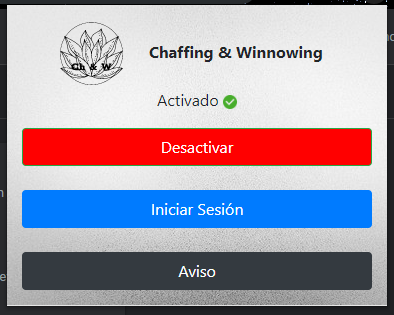
\includegraphics[width=6cm]{./imagenes/Inicio_sesion/UI_extension.png}}
          \subfloat[Extensión Habilitada]{
           \label{f:ExtensionDisabled}
            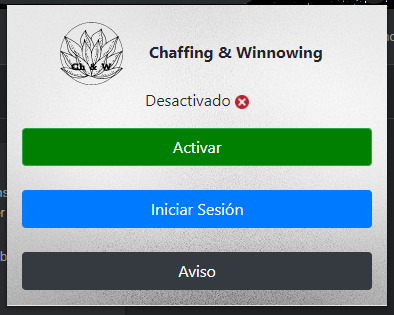
\includegraphics[width=6cm]{./imagenes/Inicio_sesion/UI_extension_disabled.png}}
         \caption[Extension habilitada / deshabilitada]{Las maneras en las que puede estar habilitada o deshabilitada la extensión}
         \label{fig:Habilitar/Deshabilitar}
         %\label{f:Enfoques}
        \end{figure}
        
        \subsection{Aviso.}
        Lo primero que se debe de realizar para que todo funcione de manera correcta es aceptar nuestro aviso de privacidad, que se encuentra en una de las opciones de la extensión; la tercera. Vamos a dar click ahí, nos aparecerá una ventana como la siguiente figura y seleccionaremos la parte de mostrar opciones avanzadas, donde escogeremos la opción de \textit{proceder a ip} y aceptemos el sitio como se muestra a continuación:
        
        \begin{figure}[H]
    		\begin{center}	
    		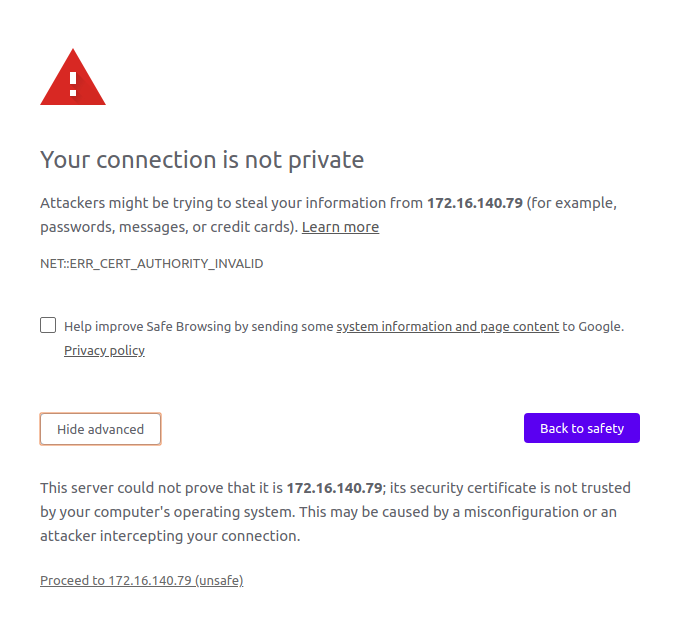
\includegraphics[width=14cm]{./imagenes/Aviso/Ext_aviso.png}
    		\caption{Pantalla de conexión no segura.}
    		\label{fig:Ext_aviso}
    		\end{center}
    	\end{figure}
        
        \begin{figure}[H]
    		\begin{center}	
    		
\includegraphics[width=12cm]{./imagenes/Aviso/Ext_avisoAccept.png}
    		\caption{Pantalla de conexión no segura.}
    		\label{fig:Ext_avisoNosegura}
    		\end{center}
    	\end{figure}
    	
    	Esto ocurre debido a que los certificados que nosotros estamos ofreciendo son autofirmados, por lo que el navegador Google Chrome detecta que no es un certificado seguro y manda esta advertencia. Una vez aceptándolo (Los pasos anteriores) no deberá haber ningún problema.
        
        \subsection{Registro de usuario.}
        Una vez que tengamos la extensión instalada y se haya aceptado el aviso de privacidad, podemos proceder a empezar a utilizarla, si es la primera vez que vamos a utilizar la extensión y no contamos con una cuenta, vamos a crear una, vamos a dar click en la extensión, nos aparecerán una serie de opciones que explicaremos más a delante, por el momento vamos a dar click en iniciar sesión.
        
        \begin{figure}[H]
    		\begin{center}	
    		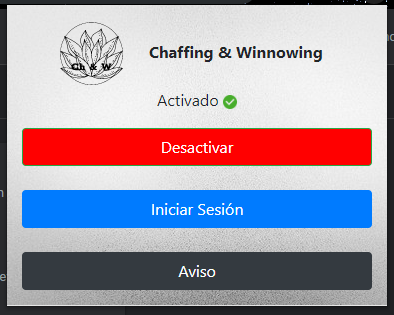
\includegraphics[width=9cm]{./imagenes/Inicio_sesion/UI_extension.png}
    		\caption{Pantalla de interfaz de la extensión.}
    		\label{fig:UI_PantallaExtension}
    		\end{center}
    	\end{figure}
    	
    	Podemos observar un pequeño esquema de como es que funciona todo este sistema, pero por ahora vamos a enfocarnos en la parte de \textit{Registrarse}, que se encuentra en la parte superior derecha de esta pestaña, vamos a dar click y nos deberá de aparecer la siguiente plantilla:
        	\begin{figure}[H]
        		\begin{center}	
        		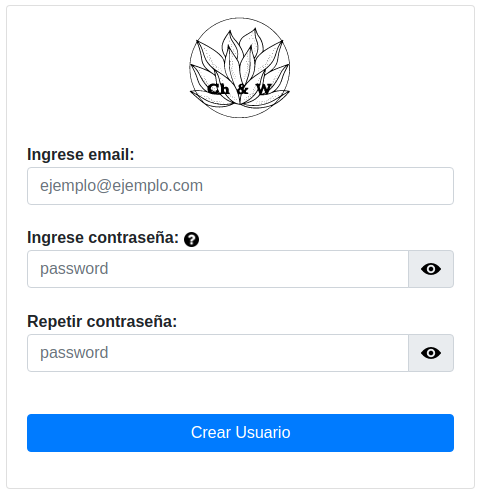
\includegraphics[width=10cm]{./imagenes/Registro/UI_registro1.png}
        		\caption{Pantalla de interfaz inicial para registro de usuario.}
        		\label{fig:UI_registo1}
        		\end{center}
        	\end{figure}
        	Vamos a llenar los datos que solicitan, esto con la finalidad de utilizar estos sencillos datos para poder generarle un certificado único.
        	\begin{figure}[H]
        		\begin{center}	
        		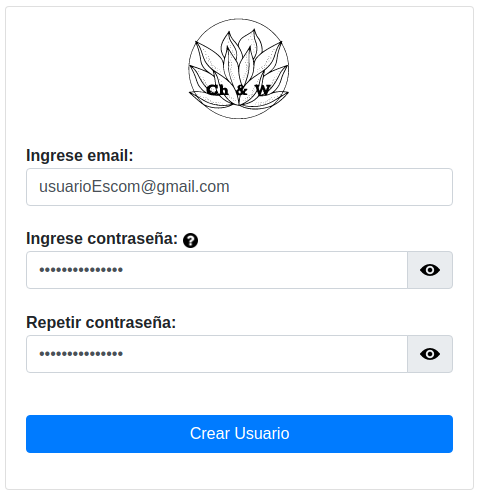
\includegraphics[width=10cm]{./imagenes/Registro/Ext_registro1.png}
        		\caption{Pantalla de interfaz para registro llenando los datos.}
        		\label{fig:Ext_registo1_llenado}
        		\end{center}
        	\end{figure}
        	
        	Si todas los datos son correctos, deberá aparecer el siguiente mensaje: 
        	
        	\begin{figure}[H]
        		\begin{center}	
        		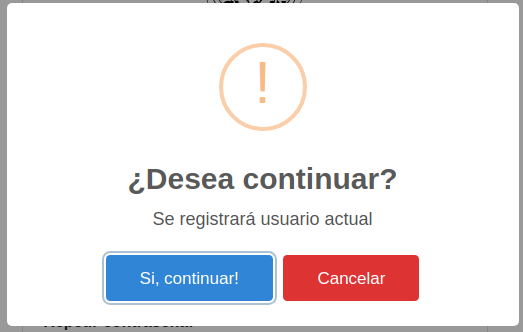
\includegraphics[width=10cm]{./imagenes/Registro/deseaContinuar.png}
        		\caption{Mensaje de confirmación de registro de usuario.}
        		\label{fig:Ext_registo1}
        		\end{center}
        	\end{figure}
        	
        	Si desea continuar con el registro, deberá dar click en ''Si, Continuar!'' si no desea continuar con el registro o cambiar algún dato introducido, seleccione la opción ''Cancelar''.\\
        	Si desea continuar, aparecerá un mensaje como el siguiente. Esto quiere decir que su cuenta ha sido creada con éxito. Al dar click en el botón ''Iniciar Sesión'' automáticamente lo llevará a la página de inicio de sesión.
        	
        	\begin{figure}[H]
        		\begin{center}	
        		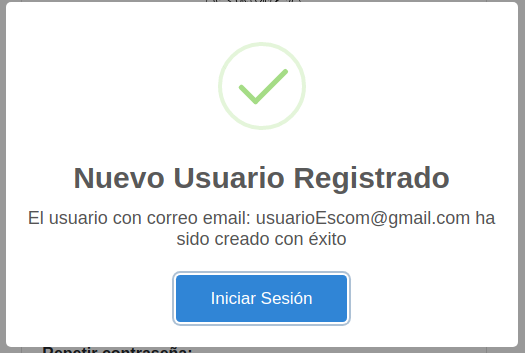
\includegraphics[width=10cm]{./imagenes/Registro/Ext_registroExitoso.png}
        		\caption{Mensaje de registro exioso.}
        		\label{fig:Ext_registoExitoso}
        		\end{center}
        	\end{figure}
    	
    	
        \subsection{Iniciar Sesión.}
        Esta opción sirve para poder identificar quien es el usuario que está utilizando la extensión en ese momento, debido a que la extensión puede ser utilizada por varios usuarios en un mismo ordenador. Como se acaba de instalar la extensión y es la primera vez que vamos a utilizarla, primero debemos de crear una cuenta (ver Registro de usuario), para esto vamos a dar click en la opción de \textit{Iniciar Sesión}, donde nos desplegará una nueva pestaña como sigue: 
        
        \begin{figure}[H]
    		\begin{center}	
    		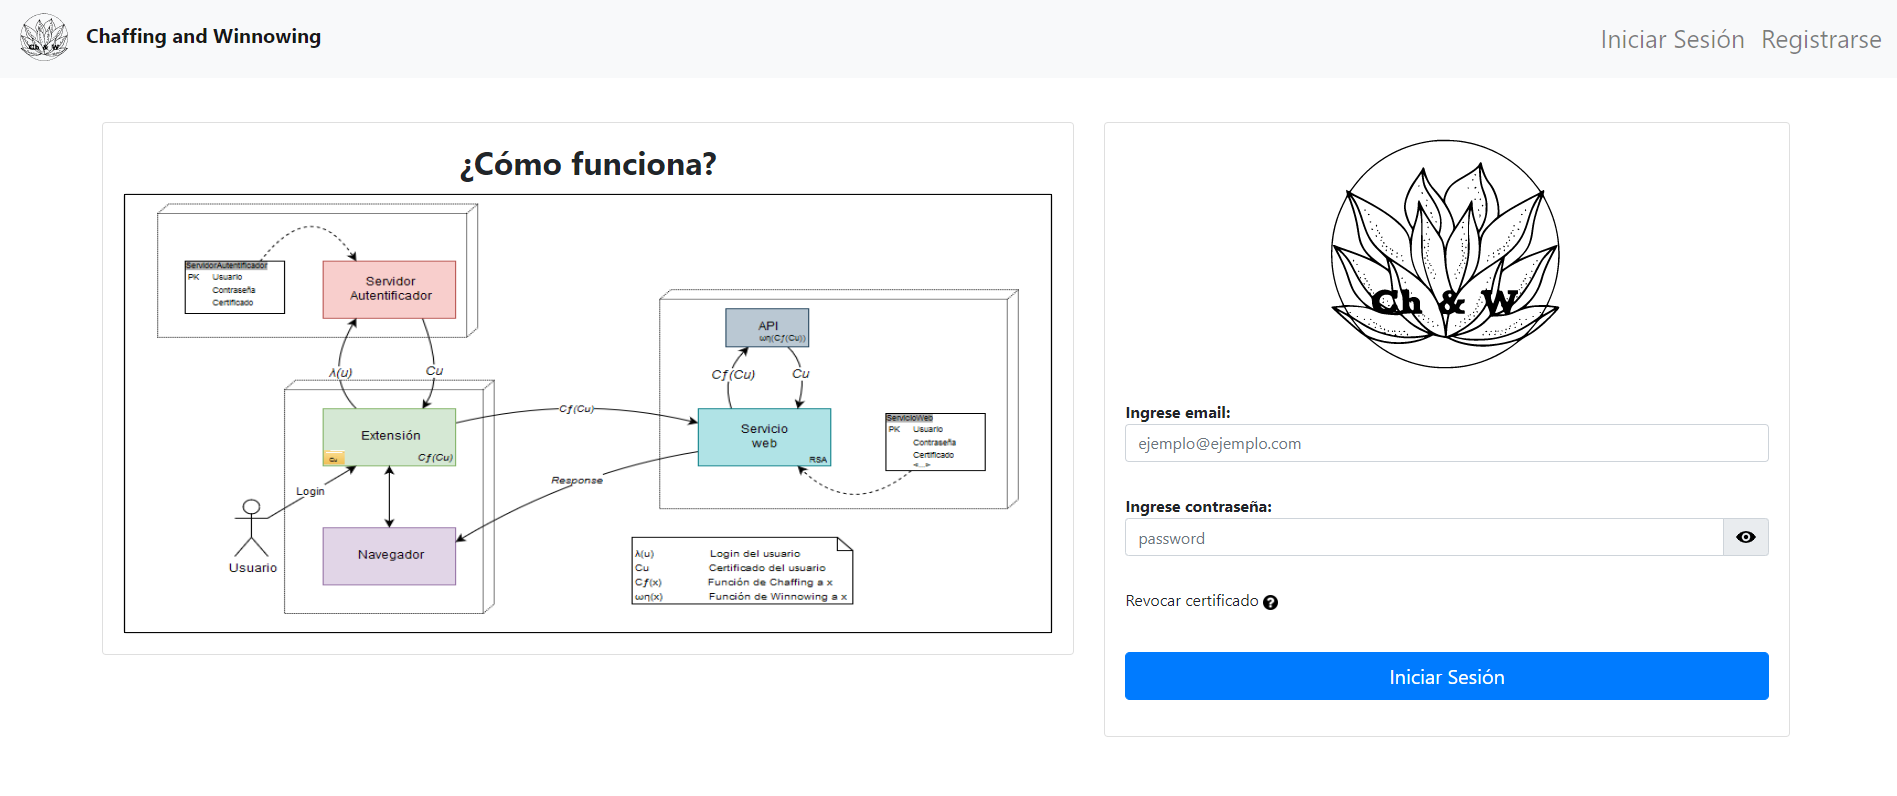
\includegraphics[width=14cm]{./imagenes/Registro/UI_inicio.png}
    		\caption{Pantalla de interfaz de la extensión.}
    		\label{fig:UI_InicioExtension}
    		\end{center}
    	\end{figure}
    	
    	
    	
    	Una vez que ya nos hemos registrado en la extensión, podemos proceder a iniciar sesión, donde los datos que tenemos que poner son el correo con el que nos registramos y la contraseña: 
    	
    	\begin{figure}[H]
    		\begin{center}	
    		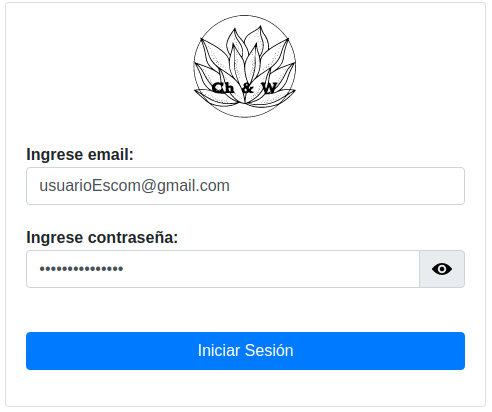
\includegraphics[width=10cm]{./imagenes/Inicio_sesion/Login.png}
    		\caption{Iniciando sesión para utilizar la extensión.}
    		\label{fig:Login}
    		\end{center}
    	\end{figure}
    	
    	Si los datos son correctos, la página nos mostrará el siguiente mensaje de éxito.
    	
    	\begin{figure}[H]
    		\begin{center}	
    		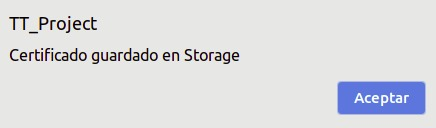
\includegraphics[width=10cm]{./imagenes/Inicio_sesion/UI_certSavedInStorage.png}
    		\caption{Iniciando sesión para utilizar la extensión.}
    		\label{fig:guardadoStorage}
    		\end{center}
    	\end{figure}
    	
    	Al dar click en Aceptar habremos concluido el proceso de inicio de sesión. Aparecerá un mensaje como el siguiente, el cual al dar click en ''Cerrar'' se cerrará la pestaña del navegador para que usted pueda navegar por la red.
        
        \begin{figure}[H]
    		\begin{center}	
    		
\includegraphics[width=10cm]{./imagenes/Inicio_sesion/graciasInicioSesion.png}
    		\caption{Mensaje de inicio de sesión concluido.}
    		\label{fig:LoginGracias}
    		\end{center}
    	\end{figure}
    	
    	Como podemos ver en la extensión, el boton de ''Iniciar Sesión'' ha desaparecido, por lo que la única opción que tiene es ''Cerrar Sesión''.
    	
    	\begin{figure}[H]
    		\begin{center}	
    		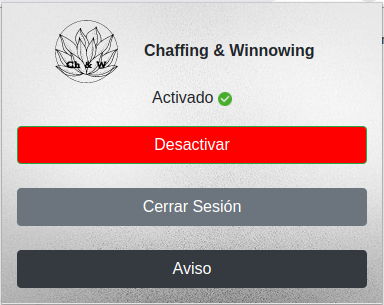
\includegraphics[width=10cm]{./imagenes/Inicio_sesion/cerrarSesionPopup.png}
    		\caption{Extensión con botón para cerrar sesión.}
    		\label{fig:cerrarSesionPopup}
    		\end{center}
    	\end{figure}
        
        \section{Utilizando la extensión.}
    Vamos ahora a utilizar la extensión, para ello es necesario asegurarnos que esta se encuentre habilitada, explicado anteriormente. Cuando la extensión se encuentra habilitada y nosotros ya tengamos la sesión iniciada podemos hacer uso de esta, para esta prueba vamos a utilizar un servicio web que nosotros mismos desarrollamos, como se muestra a continuación.
    
    \begin{figure}[H]
		\begin{center}	
		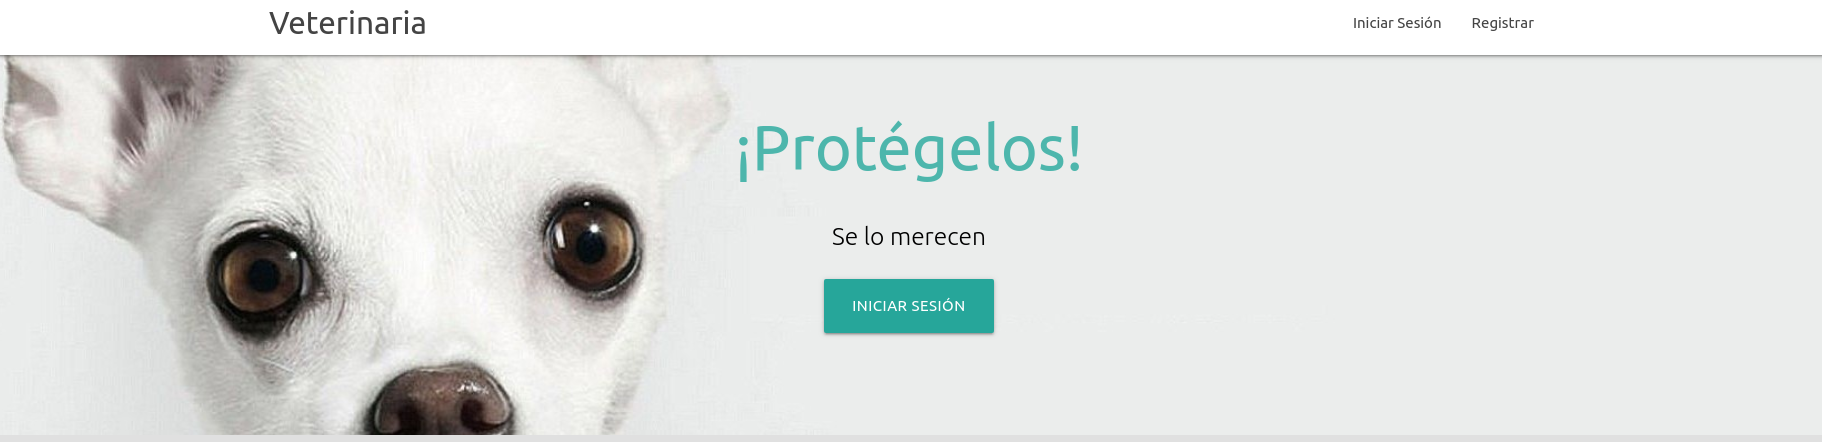
\includegraphics[width=12cm]{./imagenes/Ejecucion/UI_homeServicioWeb.png}
		\caption{Página de inicio del servicio web de prueba.}
		\label{fig:homeServicioWeb}
		\end{center}
	\end{figure}
	
	Vamos a registrarnos con una cuenta nueva, dando click en la opción de \textit{Registrar} de la página. 
	
	\begin{figure}[H]
		\begin{center}	
		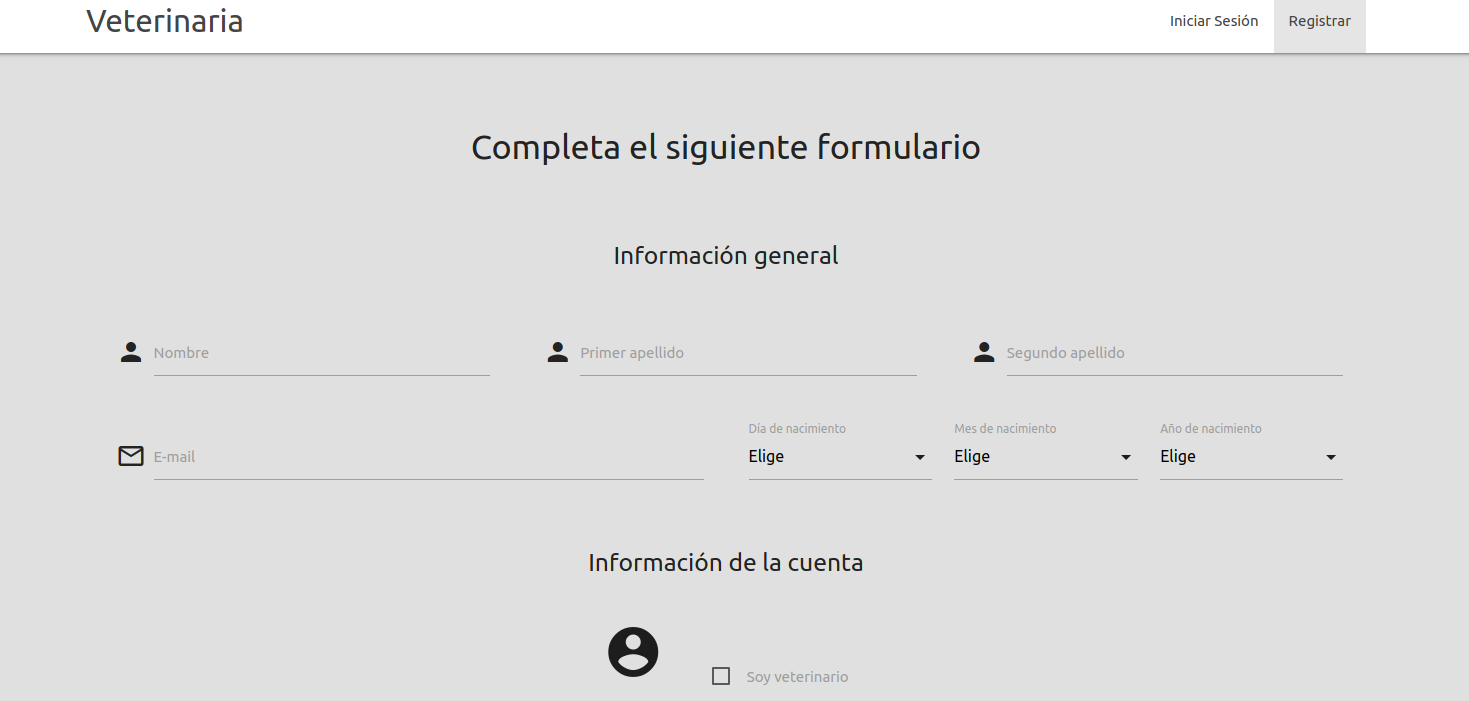
\includegraphics[width=14cm]{./imagenes/Ejecucion/UI_nuevoUsuarioServicioWeb.png}
		\caption{Página para registrarse en el servicio web.}
		\label{fig:registroNuevoUsuario}
		\end{center}
	\end{figure}
	
	Cabe resaltar el siguiente detalle, si la extensión se encuentra deshabilitada, el inicio de sesión se mostrará de la siguiente forma.
    
    \begin{figure}[H]
		\begin{center}	
		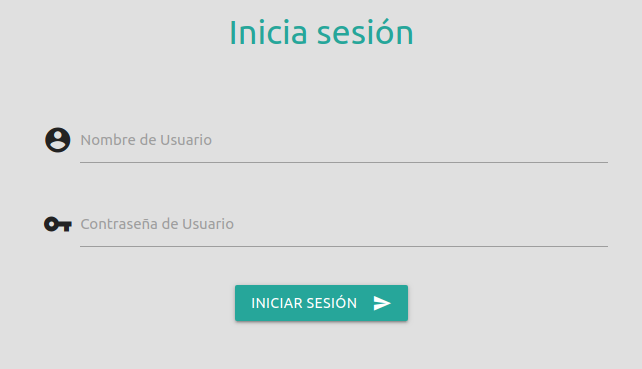
\includegraphics[width=12cm]{./imagenes/Ejecucion/UI_inicioSesionComun.png}
		\caption{Página de inicio de sesión con la extensión deshabilitada.}
		\label{fig:inicioSesionComun}
		\end{center}
	\end{figure}
	
	Si usted habilita la extensión e inicia sesión en la misma, cuando navegue en el servicio e inicia sesión, aparecerá de la siguiente manera.
	
	\begin{figure}[H]
		\begin{center}	
		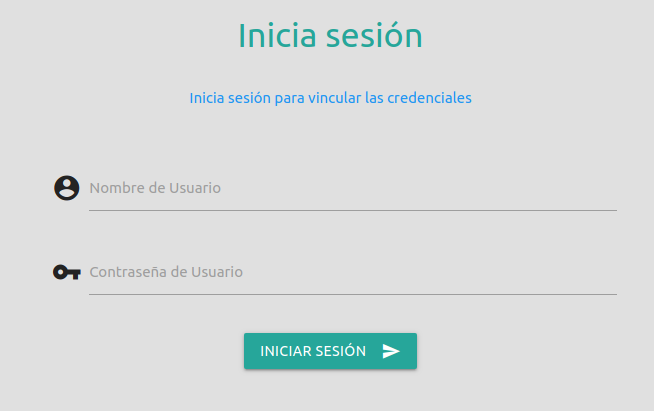
\includegraphics[width=12cm]{./imagenes/Ejecucion/UI_iniciarSesionChaffing.png}
		\caption{Página de inicio de sesión con la extensión habilitada.}
		\label{fig:iniciarSesionChaffing}
		\end{center}
	\end{figure}
    
    La extensión detecta que es la primera vez que se está ingresando en la página, por lo que solicita que se ingresen las credenciales de este servicio para así asociarle el certificado del usuario que tiene la extensión a este servicio. Una vez que inicie sesión en el servicio web, cuando usted cierre su sesión y quiera volver a ingresar a su cuenta en el servicio, tendrá acceso inmediato sin la necesidad de ingresar nuevamente sus credenciales:
    
    \begin{figure}[H]
		\begin{center}	
		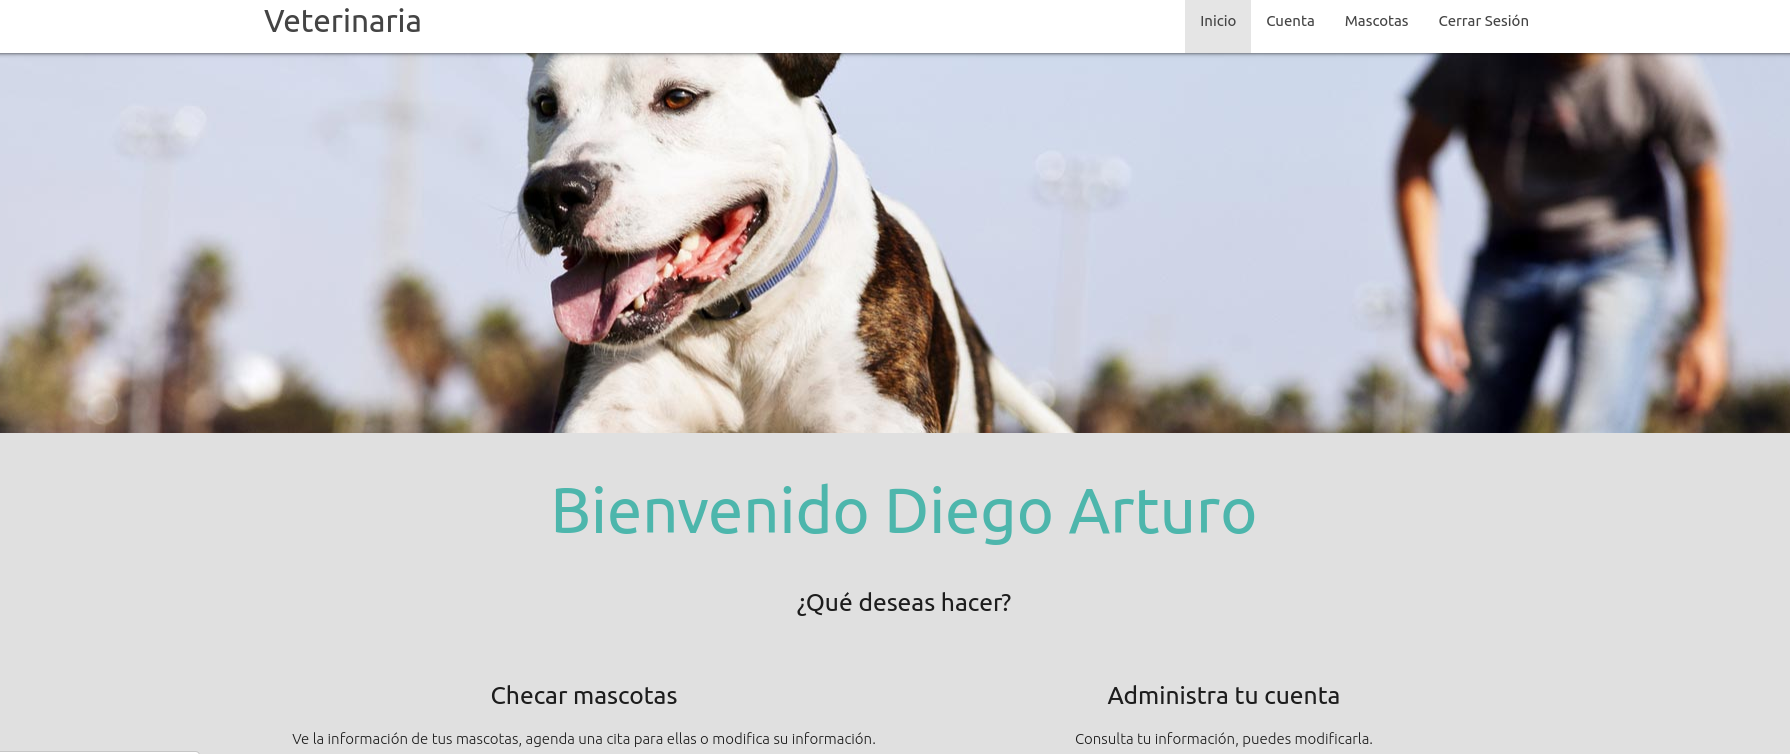
\includegraphics[width=12cm]{./imagenes/Ejecucion/UI_homeUsuario.png}
		\caption{Página de la cuenta del usuario accediendo mediante la extensión.}
		\label{fig:homeUsuario}
		\end{center}
	\end{figure}
	
	\subsection{Revocar Certificado.}
        La extensión ofrece una opción para el usuario en el que puede revocar su certificado, esto es hacer que el Servidor Autentificador pueda darte un nuevo certificado y con esto poder garantizar que el certificado que tienes en ese momento es el más actual. Esto con la finalidad de proteger mejor tus cuentas en caso de que se quedara alguna sesión abierta en algún lugar que no recordaste cerrar la sesión o que no recuerdas si la dejaste abierta o no. Para ello vamos a ir a la extensión, en la parte de Iniciar Sesión, está la opción de \textit{revocar certificado}, vamos a dar click ahí y vamos a ver que nos pide iniciar sesión, para poder saber a que usuario va a reasignar el certificado nuevo.\\
        
        Iniciamos sesión y con esto nos dirá que el certificado ha sido revocado: 
        \begin{figure}[H]
    		\begin{center}	
    		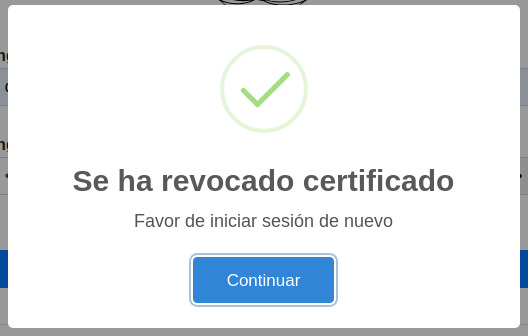
\includegraphics[width=10cm]{imagenes/Revocacion/certRevocado.jpg}
    		\caption{Certificado Revocado en la extensión.}
    		\label{fig:certRevocado}
    		\end{center}
    	\end{figure}
    	
    	Ahora si intentamos ingresar al Servicio Web de otra computadora donde tiene el certificado "anterior", no le dará acceso debido a que el certificado ya no es válido: 
    	\begin{figure}[H]
    		\begin{center}	
    		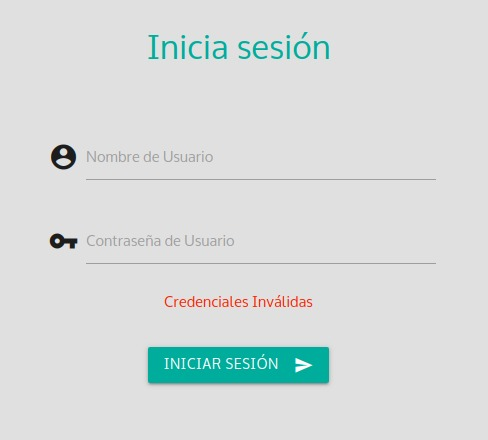
\includegraphics[width=10cm]{imagenes/Revocacion/loginNoValido.jpg}
    		\caption{Login no válido por el certificado revocado.}
    		\label{fig:loginNoValido}
    		\end{center}
    	\end{figure}
    
    %\section{Revocar certificado.}
    
    \section{Errores.}
    Es posible que el sistema mande algunos mensajes de error dependiendo de las entradas o el tipo de uso que se le de a la extensión.. Para tener un mejor control de lo que ocurre con estos errores, vamos a mostrar los más relevantes y como se pueden evitaa continuación: 
    
        \subsection{Email incorrecto.}
        Este error se da cuando el email que se ingresa no se encuentra registrado en el Servidor Autentificador. Reomendamos que verifique el correo que haya escribo.
        \begin{figure}[H]
            \centering
            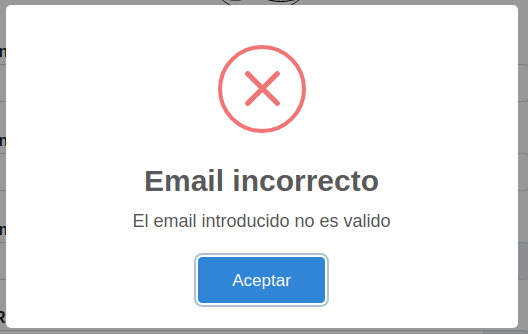
\includegraphics[width=10cm]{imagenes/Registro/emailIncorrecto.png}
            \caption{Mensaje de error al ingresar mal el correo.}
            \label{fig:emailIncorrecto}
        \end{figure}
        
        \subsection{Contraseña incorrecta.}
        Existen algunos mensajes de error relacionados con las contraseñas que se ingresan:\\
        
        La primera es cuando la contraseña que se ingresa al momento de querer iniciar sesión y se haya ingresado erroneamente la contraseña: 
        \begin{figure}[H]
            \centering
            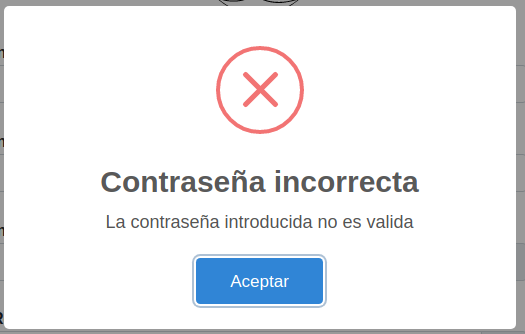
\includegraphics[width=10cm]{imagenes/Registro/contraseniaIncorrecta.png}
            \caption{Mensaje de error al ingresar la contraseña incorrecta.}
            \label{fig:contraseniaIncorrecta}
        \end{figure}
        
        La segunda es cunado, al momento de estarse registrando en la extensión, coloquemos dos contraseñas que no coinciden, esto nos arrojará el siguiente mensaje.
        \begin{figure}[H]
            \centering
            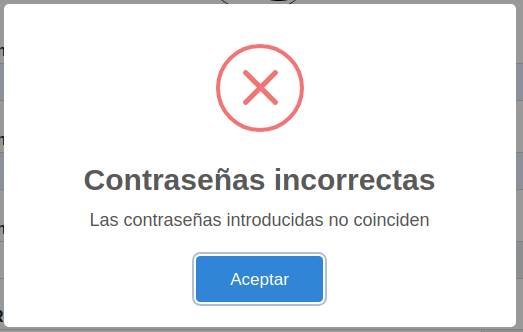
\includegraphics[width=10cm]{imagenes/Registro/UI_contraseniasNoIguales.png}
            \caption{Mensaje de error al registrarse con contraseñas diferentes.}
            \label{fig:contraseniasNoIguales}
        \end{figure}
        Para ambos casos se sugiere que se escriba la contraseña de manera tranquila para evitar cualquier error de dedo lo más posible.
        
        \subsection{Usuario no registrado.}
        Este mensaje ocurre cuando el usuario intenta iniciar sesión con una cuenta que aún no se encuentra registrada en la Autoridad Certificadora, despliega el siguiente mensaje:
        
        \begin{figure}[H]
            \centering
            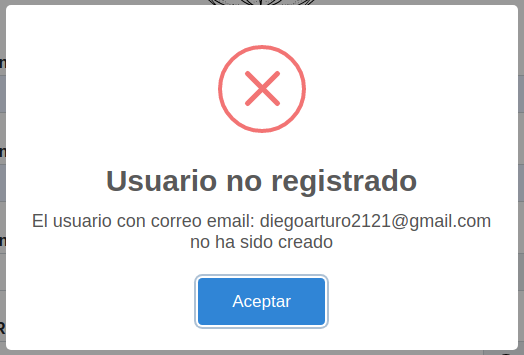
\includegraphics[width=10cm]{imagenes/Registro/usuarioNoRegistrado.png}
            \caption{Mensaje de error de usuario no encontrado.}
            \label{fig:usuarioNoRegistrado}
        \end{figure}
        
        Para evitar este error, se recomienda que al momento de escribir la cuenta, ya sea tanto para registrarse como para iniciar sesión, se verifique que en efecto sea el correo electrónico correcto.

\end{document}


